Para o desenvolvimento do trabalho serão utilizados alguns componentes externos,
tanto de \emph{hardware} quanto de \emph{software}. Será utilizado o computador
\emph{Raspberry Pi} e seu módulo de camera. Será utilizada a linguagem de programação
\emph{Python}. Será utilizada a biblioteca de visão computacional \emph{OpenCV}
juntamente com outras bibliotecas auxiliares que permitam integrar o \emph{OpenCV}
com a linguagem de programação \emph{Python} e o módulo de camera do \emph{Raspberry Pi}.
E também será utilizada a ferramenta de reconhecimento ótico de caracteres \emph{Tesseract}.

\section{Raspberry Pi}
\label{sec:raspi}

\begin{figure}[H]
	\centering
	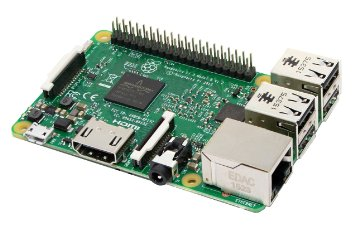
\includegraphics[width=88mm]{raspberrypi.jpg}
	\caption{O Raspberry Pi 3 model B}
	\label{fig:raspberrypi}
\end{figure}

Raspberry Pi é um computador construído em uma placa de circuito do tamanho de
um cartão de crédito desenvolvido pela Raspberry Pi
Foundation\footnote{https://www.raspberrypi.org/}. Existem diversos modelos
diferentes de Raspberry Pi no mercado, o que será utilizado no trabalho é um dos
mais recentes atualmente, o Raspberry Pi 3 model B. Será utilizado o sistema
operacional \emph{Raspbian}, que é o sistema operacional oficial suportado pela
\emph{Raspberry Pi Foundation}.

Apesar de novo, o computador ainda tem suas limitações, com um processador
quad-core ARMv8 de 1.2GHz e apenas 1GB de memória RAM\@. Pela limitação do
\emph{hardware} é possível que algumas aplicações fiquem mais lentas do que
ficariam em um computador mais potente, mas, apesar disso, o Raspberry Pi é um
computador bem completo e capaz de exercer todas as funções de um computador
normal.

O modelo utilizado de Raspberry Pi contém módulo de WiFi embutido, sem a
nescessidade de periférico, que será utilizado no trabalho para enviar as
informações processadas pela Internet. Também será utilizado um módulo externo
de câmera para coletar as imagens em tempo real.

\section{OpenCV}
\label{sec:opencv}

OpenCV (\emph{Open Source Computer Vision Library}) é uma biblioteca \emph{open
source} de visão computacional e aprendizado de máquina. Contém mais de 2500
algoritmos otimizados nessas áreas, incluindo algoritmos clássicos e recentes. A
biblioteca é escrita nativamente em C++, e dispõe de interfaces para C, C++,
Python, Java e MATLAB, suportando os sistemas operacionais Windows, Linux,
Android e Mac OS.\footnote{http://opencv.org/}

No desenvolvimento deste trabalho será utilizada a linguagem de programação \emph{Python},
e algumas bibliotecas são utilizadas para trabalhar com \emph{OpenCV}. A biblioteca
\emph{numpy}\footnote{http://www.numpy.org/}, é uma biblioteca de computação cientifica em
\emph{Python}, que inclui funções de processamento numérico e vetores que são utilizados
pelo \emph{OpenCV} para representar as imagens.

Também será utilizada o pacote \emph{picamera}\footnote{https://picamera.readthedocs.io/en/release-1.12/},
que possui uma interface em \emph{Python} para se comunicar com o módulo de camera do \emph{Raspberry Pi}.
É possível utilizar as funções próprias de captura de imagem da camera do \emph{OpenCV}, como por exemplo
o \texttt{cv2.VideoCapture(0)}, mas será optado por utilizar o \emph{picamera}, por ser uma interface mais
específica para a camera utilizada.

Um exemplo de código de captura de imagem utilizando a camera do \emph{Raspberry Pi} em \emph{Python}, utilizando
as bibliotecas citadas pode ser visto abaixo. No exemplo, os quadros são capturados pela camera do \emph{Raspberry Pi},
convertidos para escalas de tons de cinza (\emph{grayscale}), e mostrados na tela, dado que haja um monitor conectado ao
computador \emph{Raspberry Pi}. Converter a imagem para \emph{grayscale} é um dos primeiros passos de pré-processamento
para iniciar o reconhecimento da placa.

\begin{verbatim}
from picamera.array import PiRGBArray
from picamera import PiCamera
import cv2

camera = PiCamera()
rawCapture = PiRGBArray(camera, size=(640, 480))

for frame in camera.capture_continuous(rawCapture, format="bgr", use_video_port=True):
	image = frame.array
	gray_image = cv2.cvtColor(image, cv2.COLOR_BGR2GRAY)
	cv2.imshow("Frame", gray_image)
	rawCapture.truncate(0)
\end{verbatim}


\section{OCR}
\label{sec:ocr}

Reconhecimento Ótico de Caracteres (\emph{Optical Character Recognition}, OCR)
consiste da conversão de textos em formato de imagem para o formato reconhecido
por máquina. É o método mais eficiente para fazer o processamento de imagem para
texto.~\cite{mohit2015designing}

Uma ferramenta conhecida de OCR é o
Tesseract\footnote{https://github.com/tesseract-ocr/tesseract}. É uma ferramenta
\emph{open source} de reconhecimento ótico de caracteres que suporta múltiplas
línguas.  É essencialmente um algoritmo de comparação de \emph{templates}, e as
amostras de caracteres podem ser auto-treinados.~\cite{ho2016intelligent} Esta
ferramenta será utilizada para fazer o reconhecimento dos caracteres neste trabalho.

Um exemplo do uso do \emph{Tesseract} na linguagem de programação \emph{Python} pode ser
visto abaixo. É nescessário utilizar uma biblioteca chamada \emph{pytesseract}, que possui
uma interface em \emph{Python} para a utilização da ferramenta. O exemplo abaixo lê uma
imagem do disco e imprime no console quais os caracteres que foram reconhecidos.

\begin{verbatim}
from PIL import Image
import pytesseract

print(pytesseract.image_to_string(Image.open('license_plate.jpg')))
\end{verbatim}

O \emph{Tesseract} pode ser treinado para reconhecer diferentes fontes e línguas. O
treinamento deve ocorrer previamente, e não enquanto executa o reconhecimento das placas.
Deverá ser coletado um significativo número de exemplos de caracteres como eles serão segmentados
pelo algoritmo, e com esse conjunto de treinamento, deve se executar a ferramenta de treinamento do
\emph{Tesseract}. Um manual de como utilizar o \emph{software} de treinamento pode ser encontrado
no repositório do \emph{Tesseract}\footnote{https://github.com/tesseract-ocr/tesseract}, onde o
\emph{software open source} está disponível.


\section{Placa de Transito Brasileira}
\label{sec:placabr}

Segundo o código de transito brasileiro~\cite{brasil1997lei}, todos os veículos
são identificados por meio de placas dianteira e traseira. Elas são
identificadas por uma tarja na parte superior contendo a sigla do estado e o
nome do município, e pelo código de identificação único, composto por três
letras, seguidas por quatro digitos, separados por um hífen.

Veículos particulares, de aluguel, oficial, de experiência, de aprendizagem e de
fabricante têm suas dimensões de 130mmx400mm e altura dos caracteres de 63mm.
Caso a placa não caiba no receptáculo ela pode ser reduzida em até 15\%. As
placas de motocicleta, motoneta, ciclomotor e triciclos autorizados tem
dimensões de 136mmx187mm e altura de caracteres de 42mm. Imagem das placas com
suas dimensões podem ser vistos nas figuras~\ref{fig:placa_carro}
e~\ref{fig:placa_moto}.

\begin{figure}[H]
		\centering
		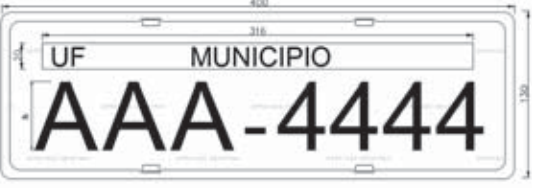
\includegraphics[width=88mm]{placa_carro.png}
		\caption{Placa de um carro}
		\label{fig:placa_carro}
\end{figure}

\begin{figure}[H]
		\centering
		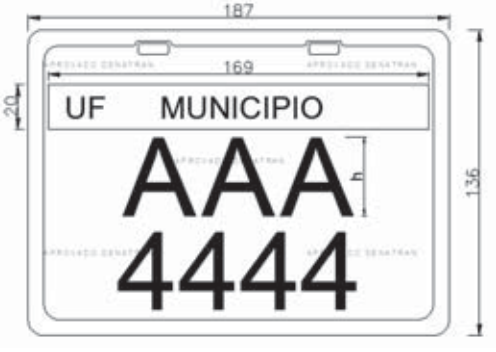
\includegraphics[width=88mm]{placa_moto.png}
		\caption{Placa de uma moto}
		\label{fig:placa_moto}
\end{figure}

A tipologia dos caracteres das placas utiliza a fonte
Mandatory~\ref{fig:tipografia}, e as placas de categorias diferentes de veículos
são diferenciadas pelas suas cores na tabela~\ref{tab:placa_cores}.

\begin{figure}[H]
		\centering
		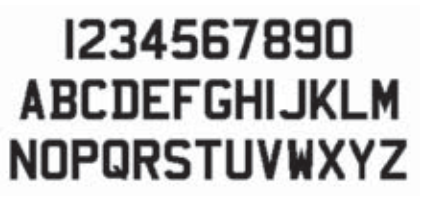
\includegraphics[width=88mm]{fonte.png}
		\caption{Tipografia das placas}
		\label{fig:tipografia}
\end{figure}

\begin{table}[]
\centering
\label{tab:placa_cores}
\caption{Cores das placas automotivas}
\begin{tabular}{|l|l|l|}
\hline
\textbf{Categoria do Veículo}                                               & \textbf{Cor de Fundo} & \textbf{Cor de Caracteres} \\ \hline
Particular                                                                  & Cinza                 & Preto                      \\ \hline
Aluguel                                                                     & Vermelho              & Branco                     \\ \hline
Experiência/Fabricante                                                      & Verde                 & Branco                     \\ \hline
Aprendizagem                                                                & Branco                & Vermelho                   \\ \hline
Coleção                                                                     & Preto                 & Cinza                      \\ \hline
Oficial                                                                     & Branco                & Preto                      \\ \hline
Missão Diplomática                                                          & Azul                  & Branco                     \\ \hline
Corpo Consular                                                              & Azul                  & Branco                     \\ \hline
Organismo Internacional                                                     & Azul                  & Branco                     \\ \hline
Corpo Diplomático                                                           & Azul                  & Branco                     \\ \hline
\begin{tabular}[c]{@{}l@{}}Organismo Consular/\\ Internacional\end{tabular} & Azul                  & Branco                     \\ \hline
\begin{tabular}[c]{@{}l@{}}Acordo Cooperação\\ Internacional\end{tabular}   & Azul                  & Branco                     \\ \hline
Representação                                                               & Preto                 & Dourado                    \\ \hline
\end{tabular}
\end{table}
